\documentclass[a4paper,12pt]{article} % тип документа

\usepackage{geometry} %геометрия страниц (отступы)
\usepackage[colorlinks=true, linkcolor=blue, urlcolor=blue]{hyperref} %ссылки

%  Русский язык
\usepackage{multirow}
\usepackage{wrapfig}
\usepackage[T2A]{fontenc}			% кодировка
\usepackage[utf8]{inputenc}			% кодировка исходного текста
\usepackage[english,russian]{babel}	% локализация и переносы
\usepackage{graphicx}
\usepackage{todonotes}

% Математика
\usepackage{amsmath,amsfonts,amssymb,amsthm,mathtools}
\usepackage{hyperref}

% графики
\usepackage{pgfplots}
\pgfplotsset{compat=1.9}

\begin{document}

\begin{titlepage}
\begin{center}
    {\large МОСКОВСКИЙ ФИЗИКО-ТЕХНИЧЕСКИЙ ИНСТИТУТ (НАЦИОНАЛЬНЫЙ ИССЛЕДОВАТЕЛЬСКИЙ УНИВЕРСИТЕТ)}
\end{center}
\begin{center}
    {\largeФизтех-школа Радиотехники и компьютерных технологий}
\end{center}

\vspace{3.5cm}

\vspace{0.1cm}
{\huge
\begin{center}
    {\bf Практикум цифрового производства}\\
    {Беспилотный летательный аппарат}
\end{center}
}
\vspace{5cm}
\begin{center}
{
    \LARGE Команда: \\ Мовсесян Михаил Б01-403 (movsesian.me@phystech.edu) \\Рогов Анатолий Б01-406 (rogov.ai@phystech.edu)
}
\end{center}

\vspace{0.5cm}
\begin{center}
    Долгопрудный 2025
\end{center}
\end{titlepage}

\newgeometry{
    left=2cm,
    right=2cm,
    top=2cm,
    bottom=2cm,
    }
\paragraph{Практикум цифрового производства. Весна 2025}
\section*{Предложение проекта: \newline Беспилотный летательный аппарат}

\paragraph{\underline{Команда}:}
Михаил Мовсесян \href{mailto:movsesian.me@phystech.edu}{\underline{movsesian.me@phystech.edu}}, Анатолий Рогов \href{mailto:rogov.ai@phystech.edu}{\underline{rogov.ai@phystech.edu}}

\paragraph{\underline{Цель проекта}:}
спроектировать и изготовить прототип БПЛА, способного летать в пределах 10 метров, с грузоподъёмностью не менее 200 г и временем полёта не менее 15 минут.

\paragraph{\underline{Задачи проекта}:}
\begin{itemize}
    \item Найти доступные на рынке электромоторы, элементы радиоаппаратуры и другие составляющие схемотехники для квадрокоптера.
    \item Определить материалы для производства деталей.
    \item Спроектировать корпус устройства под имеющиеся компоненты управления.
    \item Изготовить детали и собрать прототип.
    \item Произвести настройку устройства.
    \item Запустить аппарат и провести серию испытаний.

\end{itemize}

\paragraph{\underline{Существующие аналоги}:}

\textbf{Open-source проекты}
\begin{enumerate}
    \item \href{https://px4.io}{PX4 Autopilot} (платформа для автономных БПЛА с открытым кодом).
    \item \href{https://ardupilot.org}{ArduPilot} (аппаратно-независимая система управления).
    \item \href{https://www.dji.com/ru}{DJI Tello EDU} (образовательный дрон с программируемым управлением, но закрытой архитектурой).
\end{enumerate}

\paragraph{\underline{Эскиз проекта}:}
\begin{center}
    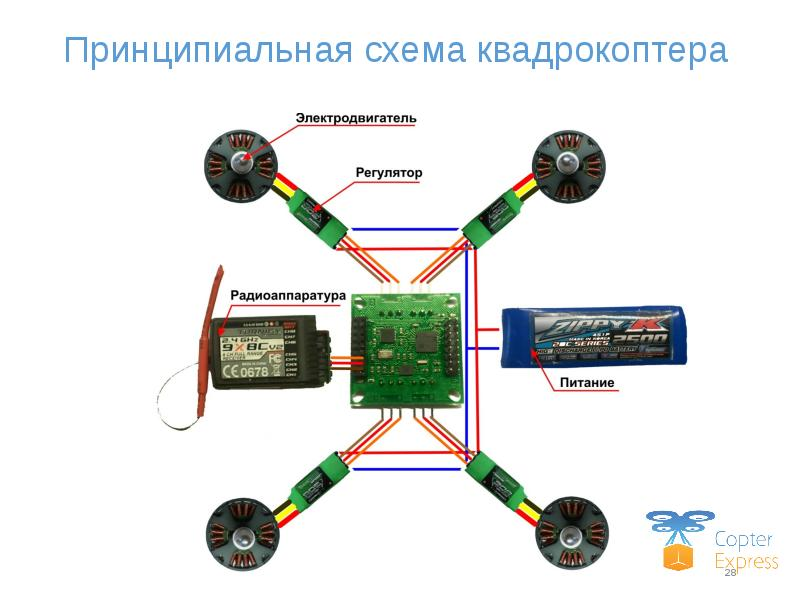
\includegraphics[width=0.7\textwidth]{img/drone.jpg} \\
\end{center}

\end{document}
